% Meta-monografia de exemplo genérico de uso da classe delaetex.cls
% Copyright (C) 2004..2016 Walter Fetter Lages <fetter@ece.ufrgs.br>
%
% This file was adapted from:
% Meta-monografia de exemplo genérico de uso da classe deletex.cls
% Copyright (C) 2004 Walter Fetter Lages <w.fetter@ieee.org>
%
% This is free software, distributed under the GNU GPL; please take
% a look in `deletex.cls' to see complete information on using, copying
% and redistributing these files
%
%\documentclass[repeatfields,openright,overleaf,nomicrotype]{tcc}
% LTeX: language=pt-BR
\documentclass[repeatfields,xlists,xpacks,oneside,yearsonly]{ufrgscca}

\graphicspath{{./img/}}
\usepackage{fancybox}
\addbibresource{TCC.bib}

\begin{document}

\maketitle

% dedicatória é opcional
%\notoc\chapter{Dedicatória} %não vai aparecer no sumário

% agradecimentos são opcionais
%\notoc\chapter{Agradecimentos}

% Agradeço ao \LaTeX\ por não ter vírus de macro\ldots

% resumo no idioma do documento
\begin{abstract}

    Neste trabalho é apresentado o embasamento teórico e o
    planejamento da implementação de mapeamento de ambientes a um
    sistema de navegação autônomo, com intuito de permitir
    o planejamento de trajetórias em um ambiente dinâmico ou
    pouco estruturado.
    Para obter este objetivo, será utilizado o ROS 2 em conjunto com o
    \textit{Navigation 2}, que será configurado para simular no Gazebo
    o robô móvel Twil, equipado de uma câmera RGB-D para mapeamento e
    localização.
    Após a verificação do sistema no ambiente simulado, será feita a
    adaptação para o robô real.
\end{abstract}

% resumo no outro idioma
% como parâmetro devem ser passadas as palavras-chave
% no outro idioma, separadas por vírgulas
% \begin{otherabstract}{Automation and Control, Robotics, SLAM}

% \end{otherabstract}

% sumario
\setcounter{tocdepth}{3}

% lista de ilustrações
\listoffigures

% lista de tabelas
\listoftables
% lista de listagens (código fonte)
%\listofcodelist %% doesn't work on overleaf

% lista de abreviaturas e siglas
% o parametro deve ser a abreviatura mais longa
\begin{listofabbrv}{PPGEE}
    \item[BT] Behavior Tree
    \item[RGB-D] Red Green Blue - Depth (vermelho verde azul - profundidade)
    \item[ROS] Robot Operating System
    \item[SLAM] Simultaneous Localization and Mapping
    \item[UFRGS] Universidade Federal do Rio Grande do Sul
\end{listofabbrv}

% lista de símbolos é opcional
% \begin{listofsymbols}{$\alpha\beta\pi\omega$}
% \end{listofsymbols}

\tableofcontents

\chapter{Introdução}

Robótica deve seu maior sucesso a indústria de manufatura, onde são utilizados
principalmente robôs manipuladores~\cite{IntroductionToMobileRobots}.
Porém, estes robôs têm como limitação sua mobilidade, incapazes de se movimentar
pela planta, limitando suas tarefas a um espaço fixo.
Um robô móvel, por outro lado, é capaz de se mover pelo seu ambiente de
trabalho, aumentando a gama de tarefas que podem ser realizadas.

Por esta razão, o mercado de robôs móveis está em crescimento, como mostra a
Figura~\ref{fig:mercado_robo}.
Estes robôs podem ser utilizados em ambientes internos, como hospitais, fábricas
ou em centros de distribuição, como o robô Proteus, da Amazon~\cite{amazon_robot}.
Esta categoria de robôs, porém, tem como desafio a navegação em ambientes dinâmicos,
muitas vezes compartilhados com humanos.
Portanto, é necessário um robô capaz de perceber seu ambiente e replanejar sua
trajetória em tempo real, de modo a evitar colisões.
%TODO: nao repetir tanto robos

\begin{figure}[htbp]
    {
        \centering
        \caption{Mercado global de robôs autônomos de 2016 a 2021, com projeção até 2028.}
        \label{fig:mercado_robo}
        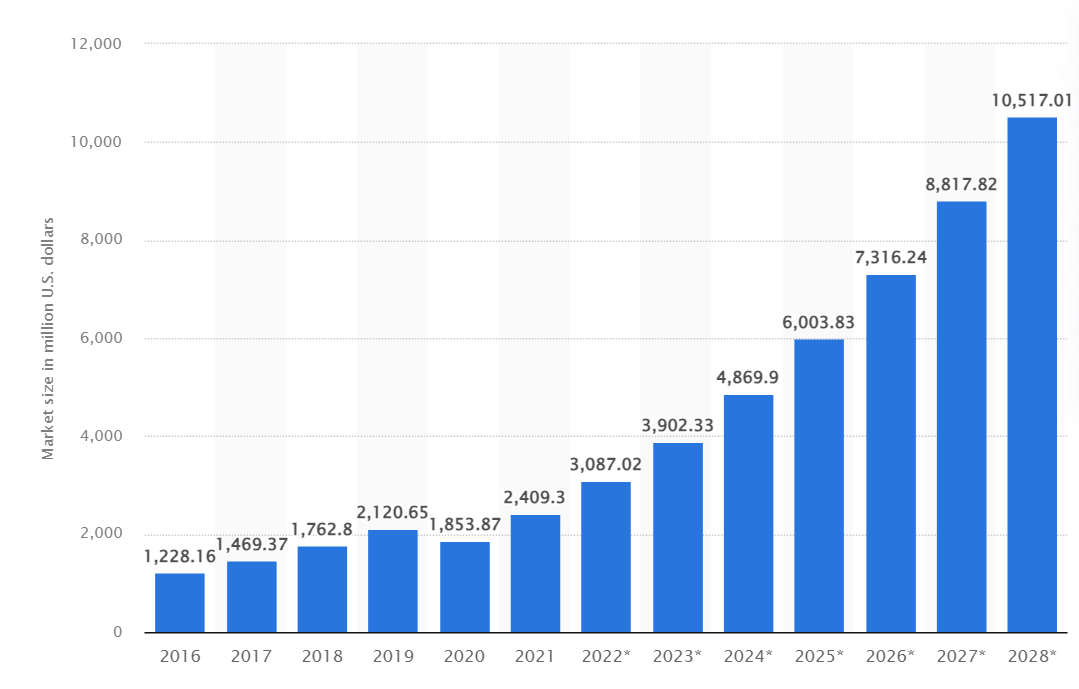
\includegraphics[width=0.9\textwidth]{mercado_robo}\\
    }
    {\sourcecitation{\textcite{robot_market}}}
\end{figure}

É neste contexto que se insere o projeto atual.
Utilizando o robô Twil, é proposto um sistema de navegação autônomo que utiliza
sensores de percepção além de algoritmos de planejamento de trajetórias para
navegar em ambientes dinâmicos ou pouco conhecidos.

Este robô já foi utilizado em trabalhos anteriores de conclusão de curso,
como em \textcite{petry_tcc} e \textcite{rahul_tcc}.
Porém, devido ao avanço do campo de robótica móvel, novas ferramentas
foram desenvolvidas, como o ROS 2 e o \textit{Navigation2}, que utilizam
técnicas modernas que serão abordadas ao longo deste trabalho.

\chapter{Revisão da Literatura}
\label{revisao}

\section{Robot Operating System 2 (ROS 2)}

O ROS 2 é a segunda geração do Robot Operating System,
um \textit{framework} para desenvolvimento de robôs.
Ele foi desenvolvido a partir do zero para atender as necessidades de robôs modernos,
com suporte para customização extensiva.
É baseado no padrão Data Distribution Service~(DDS), que é um padrão de comunicação utilizado
em sistemas de infraestrutura crítica, como sistemas militares e financeiros~\cite{ROS2Article}.

Uma mudança relevante a este trabalho do ROS 2 é nos padrões de comunicação.
Existem três tipos de comunicação no ROS 2: \textit{topics}, \textit{services} e \textit{actions}.
\textit{Topics} são canais de comunicação unidirecionais, em que um nó publica uma mensagem
e outros nós podem se inscrever para receber essa mensagem.
\textit{Services} funcionam de forma cliente servidor, utilizando o padrão de requisição e resposta.
\textit{Topics} e \textit{services} já existiam no ROS 1.

\textit{Actions}, por outro lado, são únicos ao ROS 2.
Este padrão de comunicação é utilizado para tarefas de longa duração,
em que o cliente envia uma requisição e o servidor responde com um \textit{feedback} periódico
durante a execução, além do resultado da tarefa ao seu término, podendo ser falha ou sucesso.
É possível cancelar a tarefa prematuramente.

\textit{Actions} podem ser usados, por exemplo, em tarefas de navegação, em que um \textit{action client}
envia uma requisição com um ponto de destino para um \textit{action server}
que responde com um \textit{feedback} contínuo da posição atual do robô e
com o resultado final.
Sua definição a torna apropriada na utilização em árvores de comportamento.

\section{Árvores de comportamento}

Árvores de comportamento, em inglês \textit{behavior trees}~(BT), foram desenvolvidas
na indústria de jogos para aplicação em inteligência artificial de personagens
não jogáveis, substituindo máquinas de estado.
Elas se destacam por sua modularidade e reatividade, porém, mantendo as funcionalidades
esperadas de uma máquina de estado~\cite{BehaviorTree}.

O funcionamento de uma árvore de comportamento ocorre através de uma série de
sinais enviados aos nós de uma árvore com uma frequência fixa.
Este nó responde com o estado atual da execução, que pode ser \textit{running},
se está em execução, \textit{success}, se atingiu o objetivo, ou \textit{failure}
nos demais casos.
Na formulação clássica, existem quatro categorias de nós de controle (\textit{Sequence},
\textit{Fallback}, \textit{Parallel} e \textit{Decorator}) e duas categorias
de nós de execução (\textit{Action} e \textit{Condition}).
A Tabela \ref{tab:bt_nodes} mostra os símbolos utilizados para representar
os nós de uma árvore de comportamento.

% LTeX: enable=false
\begin{table}[htb]
    \begin{center}
        \caption{Símbolos dos nós de uma árvore de comportamento.}
        \label{tab:bt_nodes}
        \begin{tabular}{cc}
            Tipo de nó         & Símbolo                    \\                    %& Sucesso                             & Falha                                & Executando                     \\
            \hline
            \textit{Fallback}  & \fbox{?}                   \\                   %& Se um filho retorna sucesso         & Se todos filhos retornam falha       & Se um filho retorna executando \\
            \textit{Sequence}  & \fbox{$\rightarrow$}       \\       %& Se todos filhos retornam sucesso    & Se um filho retorna falha            & Se um filho retorna executando \\
            \textit{Parallel}  & \fbox{$\rightrightarrows$} \\ %& Se $\geq M$ filhos retornam sucesso & Se $ > N - M$ retornam falha         & Nos outros casos               \\
            \textit{Action}    & \fbox{texto}               \\               %& Se atinge o objetivo                & Se não é possível atingir o objetivo & Durante execução               \\
            \textit{Condition} & \ovalbox{texto}            \\            %& Se é verdade                        & Se é falso                           & Nunca                          \\
            \textit{Decorator} & $\Diamond$                 \\                 %& Customizado                         & Customizado                          & Customizado                    \\
            \hline
        \end{tabular}
    \end{center}
    {\sourcecitation{Elaborado pelo autor}}
\end{table}
% LTeX: enable=true

O resultado dos nós de controle dependem dos resultados de seus nós filhos.
Por exemplo, o nó \textit{Sequence} executa seus filhos em ordem até encontrar um
nó que retorna \textit{failure} ou \textit{running}.
Caso não encontre, retorna \textit{success}.
O nó \textit{Fallback} funciona de forma semelhante porém procura filhos que retornem
\textit{success} ou \textit{running}, só retornando \textit{Failure}, caso contrário.
O nó \textit{Parallel}, executa todos os filhos em paralelo, com o resultado dependendo
do estado de execução dos filhos.
O nó \textit{Decorator} modifica o resultado de um nó filho de acordo com uma regra
definida pelo usuário.

O nó de execução \textit{Action} executa um comando, e retorna o resultado final deste comando,
como \textit{sucess} caso o objetivo seja atingido, ou \textit{failure}, caso contrário.
Enquanto a tarefa está sendo executada, o nó retorna \textit{running}.
Finalmente, o nó \textit{Condition} testa uma condição e retorna
\textit{success} ou \textit{failure}, se o resultado
for verdadeiro ou falso, respectivamente.

Estes nós podem ser combinados para facilmente criar comportamentos
procurados em robôs, como mostra a Figura \ref{fig:bt_exemplo},
que descreve a operação de \textit{pick-and-place} de um robô manipulador móvel,
utilizando os nós \textit{Fallback}, \textit{Condition},
\textit{Sequence} e \textit{Action}.

\begin{figure}[htbp]
    {
        \centering
        \caption{Exemplo de árvore de comportamento de um robô manipulador móvel.}
        \label{fig:bt_exemplo}
        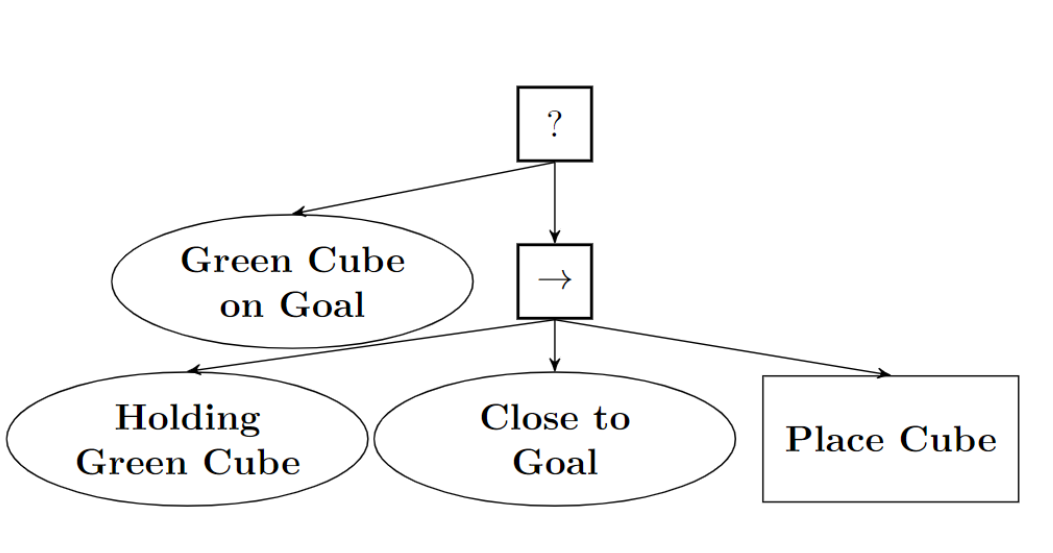
\includegraphics[width=0.5\textwidth]{bt_exemplo.png}\\
    }
    {\sourcecitation{\textcite{BehaviorTree}}}
\end{figure}

Como permitem a construção destes comportamentos de forma visual, sem a
necessidade de programação, árvores de comportamento estão sendo cada
vez mais utilizadas em projetos de robótica. Exemplos de produtos
reais são o robô JIBO e o projeto iQmatic da Scania, que
utiliza árvores de comportamento no sistema de navegação de caminhões
autônomos~\cite{BehaviorTree}.

\section{Mapeamento}

Para navegação autônoma, o robô deve ter conhecimento prévio do ambiente
para planejamento de trajetórias.
Existem diversas formas de representação do ambiente,
como mapas de gradientes, mapas de custo e vetores de espaços.
Neste trabalho, o foco será no mapa de custo.

O mapeamento também auxilia na localização do robô, comparando o mapa construído
com os dados dos sensores em tempo real. Além disso, os dados dos sensores podem ser
utilizados para atualizar o mapa de custo, em casos de ambientes pouco conhecidos ou dinâmicos.

É possível utilizar os dados de localização e dos sensores para construir um novo mapa.
Esta técnica é conhecida como \textit{Simultaneous Localization and Mapping~(SLAM)},
que permite a criação de mapas para ambientes pouco ou não conhecidos.

\subsection{Mapas de custo}

Um mapa de custo é uma representação de ambiente composta por uma
grade de células que contém um valor, variando de desconhecido, livre,
ocupado ou custo inflado.

Em mapas de custo tradicionais, seus dados são armazenadas em mapas monolíticos,
para utilização em planejamento de trajetórias.
Esta implementação é utilizada com sucesso para caminhos curtos,
mas pode apresentar dificuldade em lidar com ambientes dinâmicos
maiores~\cite{layered_costmaps}.

Uma solução para este problema são mapas de custo com camadas,
que separam o processamento dos dados dos mapas de custos em camadas semanticamente distintas.
Por exemplo, os dados dos sensores e o mapa estático previamente conhecido são processados
em camadas separadas e depois combinados em um único mapa de custo.
A Figura \ref{fig:mapa_camadas} mostra uma configuração possível de camadas
de mapas de custo.

\begin{figure}[htbp]
    {
        \centering
        \caption{Exemplo de configuração de camadas de um mapa de custo.}
        \label{fig:mapa_camadas}
        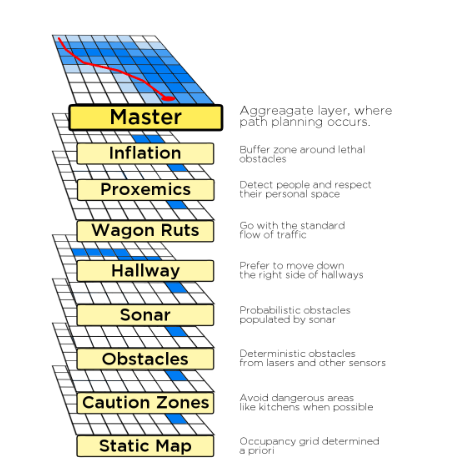
\includegraphics[width=0.5\textwidth]{mapa_camadas.png}\\
    }
    {\sourcecitation{\textcite{layered_costmaps}}}
\end{figure}

\subsection{Sensores e SLAM}

A escolha do sensor é importante para o mapeamento,
pois afeta a qualidade e quantidade de informações obtidas pelo robô, além
de determinar a escolha das ferramentas utilizadas para o mapeamento do
ambiente~\cite{SensorAndSLAM}.

Sensores acústicos, como sonares e sensor de distância a laser, são utilizados
em ferramentas SLAM 2D tradicionais. Estes sistemas são robustos e bem estabelecidos,
com fácil integração ao sistema de navegação do ROS 2.

Porém, com o avanço da tecnologia, sensores RGB-D e câmeras estéreo estão se tornando
mais acessíveis, influenciando o desenvolvimento de sistemas de Visual~SLAM~(VSLAM).
Dentre sistemas de VSLAM, destacam-se o ORB-SLAM3, OpenVSLAM e RTABMap, que possuem suporte
a câmeras RGB-D e permitem localização pura.
Em \textcite{VSLAM}, é feita uma comparação entre estes sistemas, mostrando que o
OpenVSLAM é a técnica mais adequada para maioria dos casos.
Contudo, para ambientes internos com câmeras RGB-D, o RTABMap também teve um bom desempenho.
Estes sistemas, porém, não são integrados nativamente ao \textit{Navigation2}.

% TODO: Procurar artigos mais novos sobre VSLAM (o referenciado ta na pagina
% do nav2, mas parece estar desatualizado...)
% O NVidia Isaac ROS VSLAM e o StellaROS(parece que é uma continuacao do OpenVSLAM)
% parecem promissores...

\section{Navigation2}

O \textit{Navigation2}~(Nav2) é o sucessor do ROS \textit{navigation stack}, permitindo
a realização de tarefas complexas em diversos ambientes e classes de robôs cinemáticos.
Baseando-se no legado do \textit{navigation stack} do ROS 1, o Nav2 foi construído em cima
do ROS2, implementando técnicas mais modernas para ter um sistema modular propício para
ambientes dinâmicos com suporte a uma maior variedade de sensores~\cite{Nav2}.

\begin{figure}[htbp]
    {
        \centering
        \caption{Arquitetura do \textit{Navigation2}}.
        \label{fig:nav2_arc}
        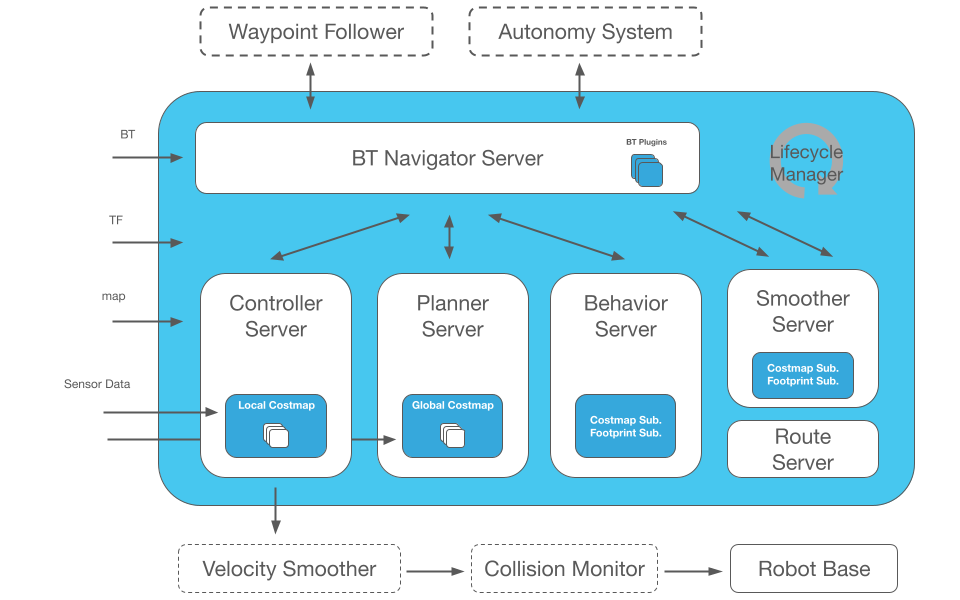
\includegraphics[width=0.9\textwidth]{nav2_architecture.png}\\
    }
    {\sourcecitation{\textcite{nav2_site}}}
\end{figure}

Na Figura \ref{fig:nav2_arc} é mostrada a arquitetura do Nav2.
O \textit{Behavior Tree~(BT) Navigator Server} usa uma árvore de comportamento para
orquestrar as tarefas de navegação, ativando os servidores de controle, planejamento e
recuperação para navegar.
Para executar nós de \textit{actions}, são normalmente utilizados
\textit{Action servers} do ROS 2.
Esta árvore de comportamento pode ser configurada pelo usuário através de um arquivo
em XML, permitindo a descrição de comportamentos de navegação únicos sem
necessidade de programação.

Além disso, todos estes servidores utilizam o conceito de \textit{Managed Nodes},
também conhecidos como \textit{Lifecycle Nodes}.
Estes nós utilizam máquinas de estados para gerenciar seu ciclo de vida, utilizando
transições de estado desde sua criação a destruição.
No caso de falha ou desligamento, o nó vai do estado ativo ao estado finalizado,
seguindo a máquina de estados, permitindo que o sistema seja interrompido
de forma segura.

Na arquitetura pode-se notar a utilização de dois mapas de custo, um local e
outro global.
O mapa local, utilizado no servidor do controlador, realiza o planejamento
a curto prazo e prevenção de colisão, enquanto o mapa global,
aplicado no servidor de planejamento, é usado principalmente
para planejamento a longo prazo.

\chapter{Metodologia}
\label{desenvolvimento}

Neste capítulo será explicado o desenvolvimento do trabalho, descrevendo o
estado atual do projeto, além de ajustes e adições planejadas para atingir
os objetivos propostos.
A maior parte do desenvolvimento do trabalho será realizada no pacote \textit{twil},
composto por diversos pacotes menores, que definem as funcionalidades do robô Twil.
Este pacote tem como dependências pacotes desenvolvidos dentro da
Universidade Federal do Rio Grande do Sul~(UFRGS), além de pacotes de
terceiros, como ROS 2 e o \textit{Nav2}.
Todos os pacotes modificados neste trabalho estão disponíveis em um repositório git
no servidor da UFRGS, onde foi criada \textit{branch} para o desenvolvimento
deste projeto.

\section{Configuração do robô}

O modelo do robô está descrito no pacote \textit{twil\_description}, que contém
os arquivos de descrição do robô no formato XACRO, que é compilado para o formato
URDF, utilizado pelo ROS 2.
A utilização do XACRO permite a criação de parâmetros, que são utilizados nos
arquivos de \textit{launch} para habilitar e desabilitar partes do robô.
Além da representação física, nestes arquivos são incluídos \textit{plugins}
do Gazebo que simulam os sensores do robô.

O sensor de percepção presente no Twil é a câmera Intel RealSense D435, que
é uma câmera RGB-D.
Para sua utilização é necessária a instalação do pacote
\textit{realsense-ros}~\cite{realsense_ros}, que contém os arquivos de
descrição da câmera, além da definição das mensagens publicadas pela mesma.
Para a simulação, foi adicionado o \textit{plugin} do Gazebo
\textit{camera\_plugin} ao arquivo de descrição do robô.
Este \textit{plugin} publica mensagens do tipo \textit{sensor\_msgs/PointCLoud2}, que
serão utilizadas para o mapeamento do ambiente.

A dinâmica do robô é implementada pelo pacote \textit{twil\_bringup},
que contém arquivos de configuração dos controladores, além de arquivos de
\textit{launch} para teste.
Os controladores estão presentes nos pacotes \textit{linearing\_controllers} e
\textit{non\_smooth\_backstep\_controller}, disponíveis no repositório da UFRGS.
Estes controladores também são responsáveis pela publicação de
informações de odometria no tópico \textit{odom}, utilizadas para localização
durante a navegação.

\section{Ambiente de simulação}

A verificação do funcionamento do sistema de navegação será feita em uma simulação
em 3D do prédio Centenário da Escola de Engenharia da UFRGS.
Utilizando o \textit{Building Editor} do Gazebo, foi criado um modelo em 3D do prédio,
tendo como base a planta do 1º andar, mostrada na Figura \ref{fig:planta_centenario}.
No pacote \textit{ufrgs\_map} está incluído uma representação em formato DWG desta
imagem, para utilização na camada estática do mapa de custo.

\begin{figure}[htbp]
    {
        \centering
        \caption{Planta do 1º andar do prédio Centenário da EE-UFRGS}
        \label{fig:planta_centenario}
        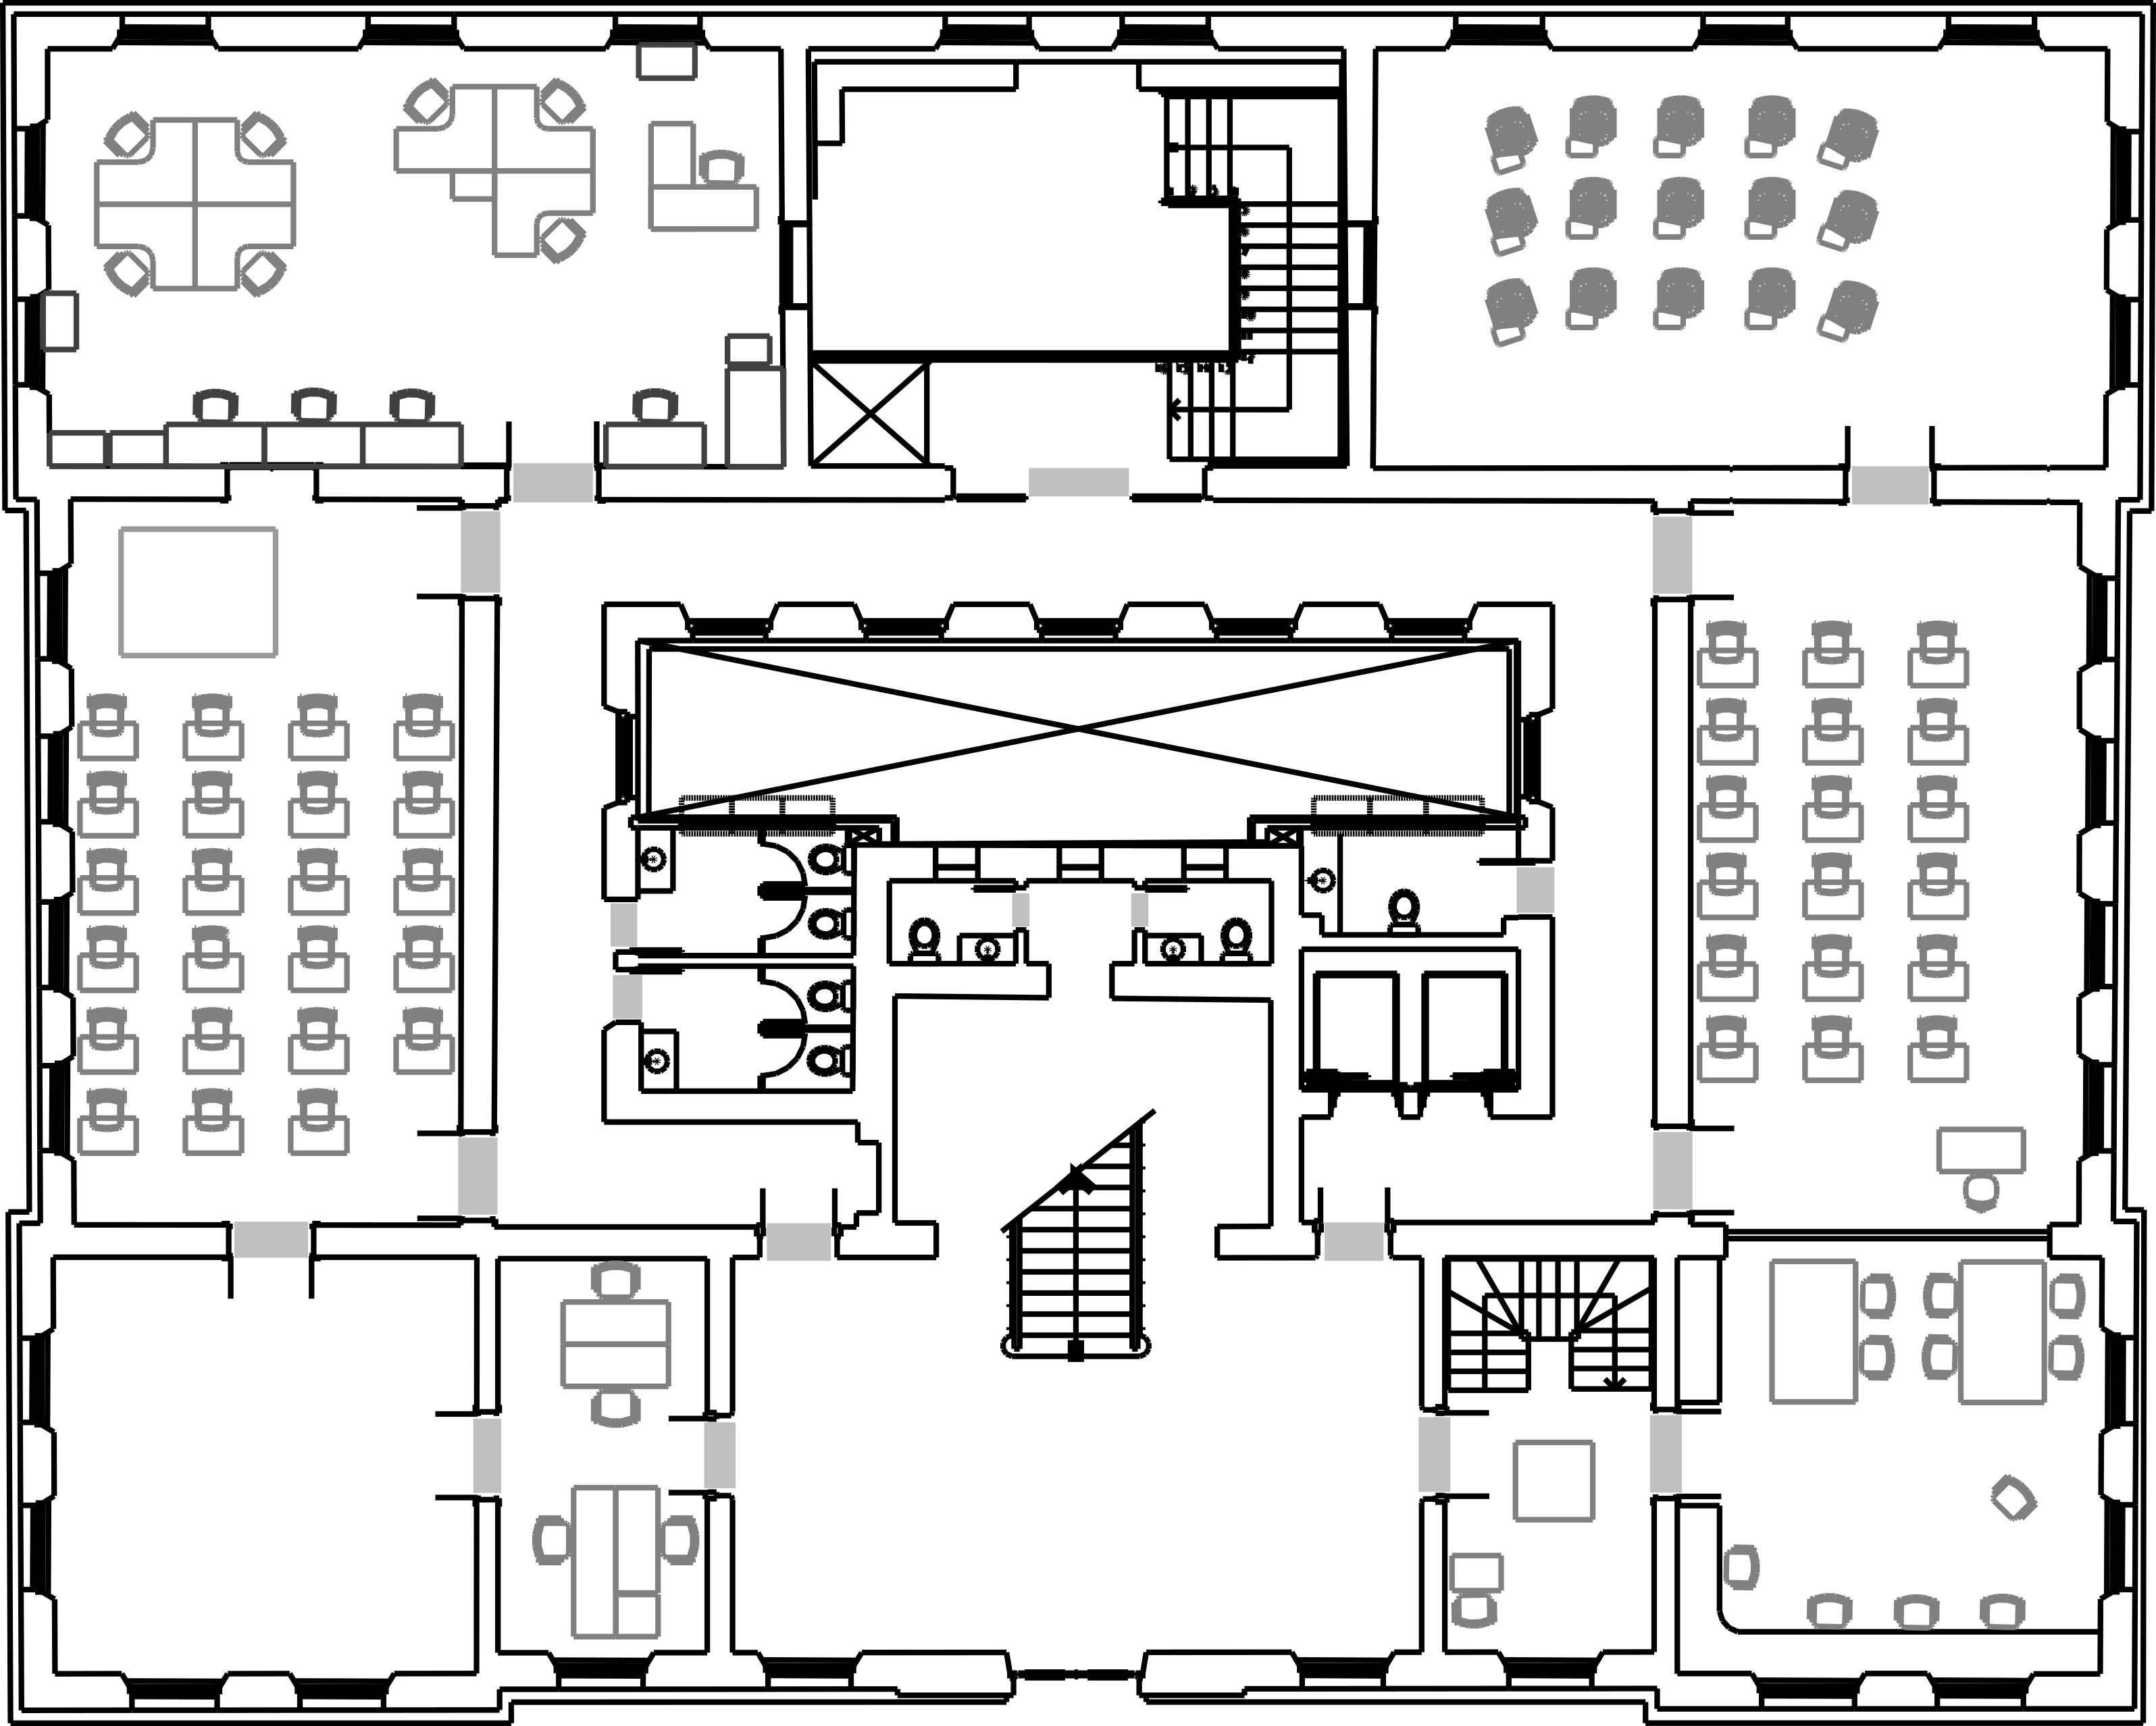
\includegraphics[width=0.5\textwidth]{centenario_floor_plan.png}\\
    }
    {\sourcecitation{\textcite{petry_tcc}}}
\end{figure}

O modelo em 3D, mostrado na Figura \ref{fig:gazebo_centenario}, faz parte do pacote
\textit{ufrgs\_gazebo}, com um arquivo \textit{world} do Gazebo,
para utilizar como ambiente de testes de navegação.
Obstáculos podem ser adicionados durante a simulação, como mesas e cadeiras,
para testar a capacidade do robô de evitar colisões.

\begin{figure}[htbp]
    {
        \centering
        \caption{Ambiente Gazebo com modelo do prédio Centenário da EE-UFRGS}
        \label{fig:gazebo_centenario}
        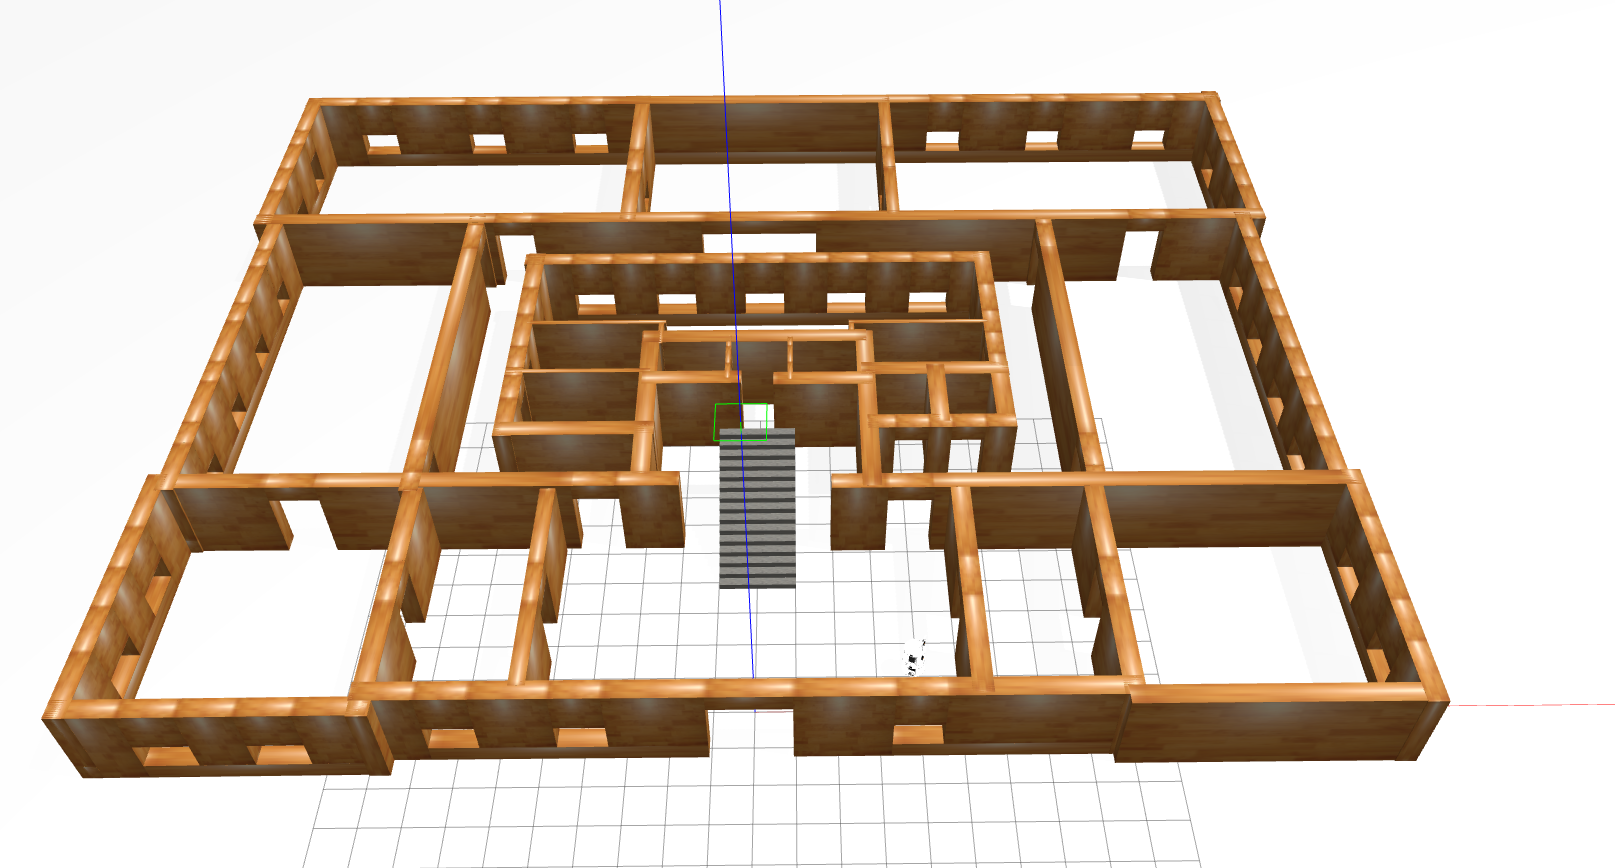
\includegraphics[width=0.9\textwidth]{gazebo.png}\\
    }
    {\sourcecitation{Autor}}
\end{figure}

\section{Configuração do Nav2}

A navegação será realizada utilizando o \textit{Navigation 2}.
A movimentação é iniciada com uma mensagem do tipo \textit{NavigateToPose},
enviada através do RViz.
O \textit{Nav2} recebe esta mensagem e, utilizando uma árvore de comportamento,
orquestra as tarefas de navegação, ativando os servidores de controle, planejamento
e recuperação para navegar até o ponto de destino.
Porém, antes de utilizar este sistema, ele deve ser configurado para o robô Twil.

\subsection{Localização}

Primeiramente, deve ser configurado o sistema de localização do robô.
Atualmente, está sendo utilizado os dados publicados pelo controlador no
tópico \textit{odom} para estimar a posição do robô.
Na Figura~\ref{fig:robo_rviz} é mostrado o robô Twil no RViz, com a representação
gráfica da trajetória real, em verde, e a trajetória estimada pelo controlador,
em vermelho.
Nota-se que a posição esperada diverge da real mais do que o esperado, portanto,
devem ser realizados ajustes nos parâmetros do controlador.

\begin{figure}[htbp]
    {
        \centering
        \caption{RViz com o robô Twil no ambiente do prédio Centenário da EE-UFRGS}
        \label{fig:robo_rviz}
        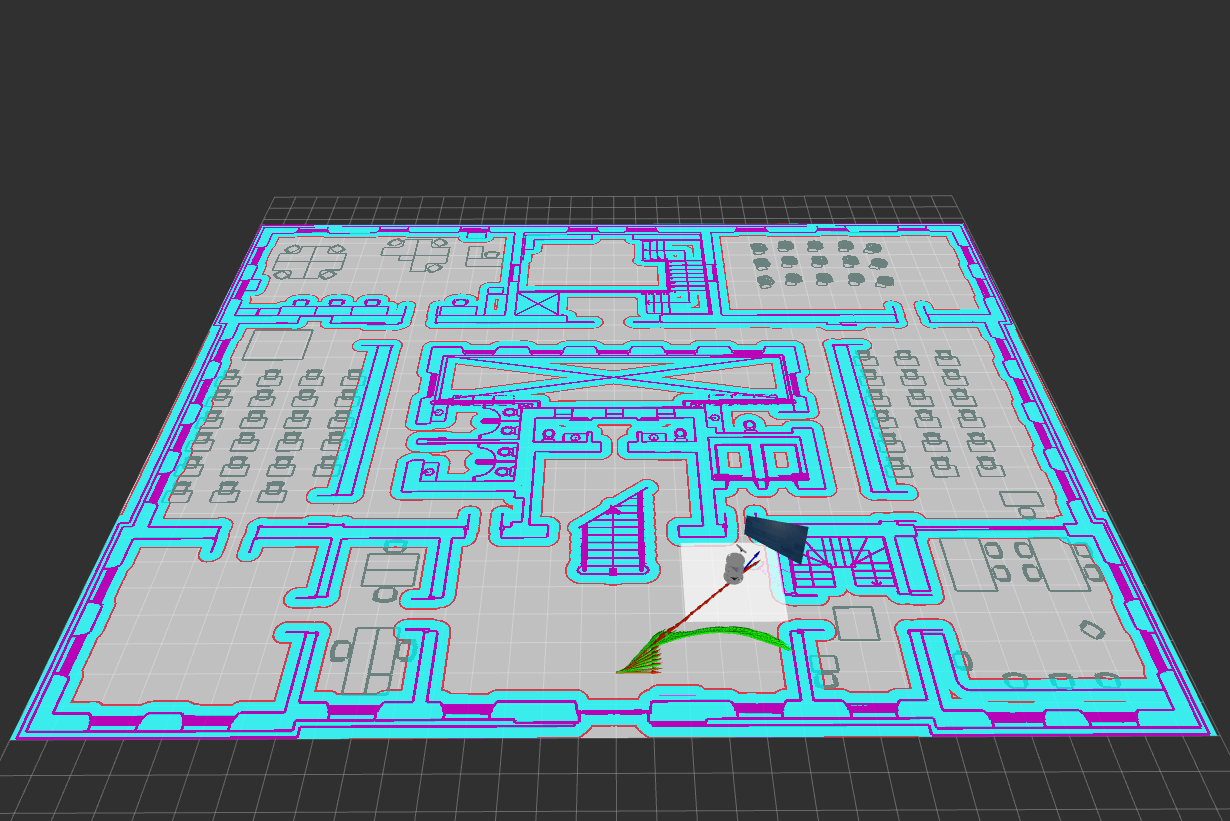
\includegraphics[width=0.8\textwidth]{erro_de_odometria.png}\\
    }
    {\sourcecitation{Autor}}
\end{figure}

Para melhorar a acurácia da localização, é possível utilizar outras fontes de
dados e, utilizando o pacote \textit{robot\_localization}, fundir os dados
através de um filtro de Kalman.
Desta forma, as desvantagens de cada sensor podem ser compensadas pelos outros
sensores.
Sensores inercias são comumente usados para esta finalidade.
Utilizando o \textit{plugin} IMU do Gazebo, ele pode ser adicionado à descrição
do robô, publicando mensagens do tipo \textit{sensor\_msgs/Imu}.


Deve ser implementada, também, a odometria visual, utilizando uma câmera RGB-D.
A odometria visual utiliza o mapa do ambiente e os dados dos sensores para estimar
a posição do robô.
Os pacotes \textit{nav2\_amcl}, \textit{slam\_toolbox}, \textit{ORB-SLAM3}
e \textit{OpenVSLAM} são capazes de realizar esta funcionalidade.
Os dois primeiros estão integrados ao \textit{Nav2},
porém foram criados para utilizar sensores LIDAR e, portanto,
necessitam de mensagens do tipo \textit{LaserScan}.
A câmera RGB-D, por outro lado, publica mensagens do tipo \textit{PointCloud2},
logo, é necessário converter estas mensagens para o tipo \textit{LaserScan}
para a utilização destes pacotes.

Em contrapartida, os pacotes \textit{ORB-SLAM3} e \textit{OpenVSLAM} foram
criados para utilizar câmeras RGB-D. Entretanto, estes sistemas não estão
integrados ao \textit{Nav2} e, devido ao caráter recente das técnicas de
VSLAM, não são tão robustos quanto os pacotes anteriores.
Desta forma, serão implementados ambos sistemas, para que seja possível
comparar os resultados de cada um.

A publicação dos dados de odometria deve seguir a norma de sistema de coordenadas
REP~105~\cite{rep_105}, utilizada pelo \textit{Nav2}.
Resumidamente, esta norma exige a existência de transformadas de \textit{map}
para \textit{odom} e \textit{odom} para \textit{base\_link}.

\subsection{Mapeamento}

A representação do ambiente no \textit{Nav2} é feita através de um mapa de custo.
As camadas do mapa são definidas através de \textit{plugins} que permitem
diversas fontes de dados para a construção do mapa.
Neste trabalho, serão utilizadas as camadas: \textit{static\_layer},
\textit{voxel\_layer}, \textit{obstacle\_layer} e \textit{inflation\_layer},
implementadas através de \textit{plugins} do \textit{Nav2}.

A camada estática, gerada pelo \textit{plugin} \textit{static\_layer},
é utilizada para representar o mapa fixo do ambiente.
Neste trabalho, será utilizada a planta do 1.º andar do prédio Centenário da EE-UFRGS,
representada na Figura \ref{fig:planta_centenario}.
Posteriormente, utilizando sistemas de SLAM, podem ser criados mapas atualizados
para utilização nesta camada.

As camadas \textit{voxel\_layer} e \textit{obstacle\_layer} utilizam dados dos
sensores de percepção para atualizar dinamicamente o mapa.
A diferença entre estas camadas é que a \textit{voxel\_layer} utiliza dados 3D
ao invés de 2D, como a \textit{obstacle\_layer}. Ambas podem utilizar mensagens
do tipo \textit{PointCloud2}, então não será necessária a conversão dos
dados provenientes da câmera RGB-D.
A inclusão destas camadas é fundamental para evitar colisões com obstáculos
ausentes no mapa estático.

A última camada, \textit{inflation\_layer}, cria uma zona de segurança ao redor
dos objetos captados nas outras camadas, para garantir uma distância segura
ao planejar a trajetória.
Em \textcite{ros_tuning_guide}, recomenda-se que a curva de inflação tenha uma
inclinação baixa, para cobrir corredores inteiros.
Desta forma, haveria preferência por caminhos que passem o mais longe possível
dos obstáculos, como mostra a Figura~\ref{fig:inflation_layer}.

\begin{figure}[htbp]
    {
        \centering
        \caption{Comparação entre curvas de inflação com inclinações baixa e alta.}
        \label{fig:inflation_layer}
        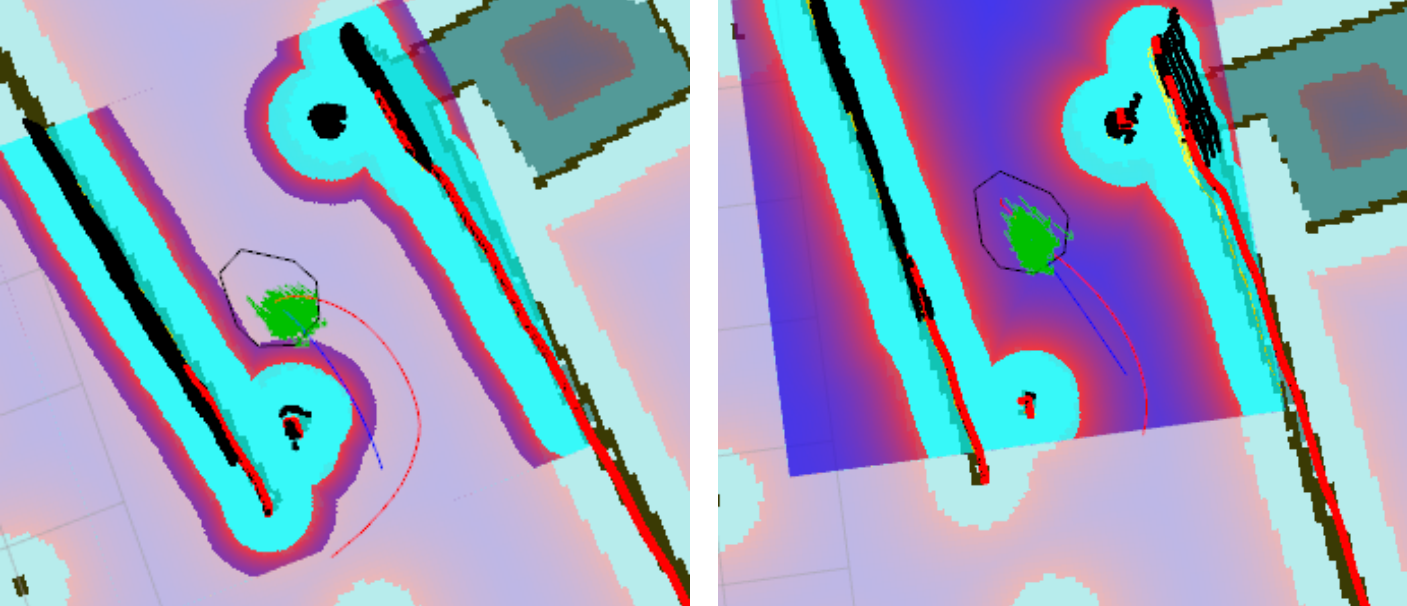
\includegraphics[width=0.8\textwidth]{inflation_layer.png}\\
    }
    {\sourcecitation{\textcite{ros_tuning_guide}}}
\end{figure}

\subsection{Planejamento de trajetórias}

Finalmente, é necessário configurar o planejamento de trajetórias.
Diversos \textit{plugins}  estão disponíveis no \textit{Nav2},
como o \textit{NavFnPlanner}, \textit{Smac Planner 2D} e \textit{Theta Star Planner}.
Neste trabalho, foi escolhido o \textit{NavFnPlanner}, que pode utilizar
os algoritmos \textit{Dijkstra} ou \textit{A*}. % TODO: ADICIONAR AS CITATIONS DO DIJKSTRA e A STAR AQUI
Este é o planejador recomendado pelos autores do \textit{Navigation 2}
para robôs circulares.

\chapter{Conclusão}
\label{conclusao}

O planejamento realizado neste trabalho evidenciou a modularidade do ROS 2,
que se tornou uma grande vantagem durante o projeto.
Um exemplo disso é a utilização de diversos pacotes de terceiros,
aproveitando o trabalho de outros desenvolvedores.
Além disso, o desenvolvimento pôde ser realizado gradualmente,
isolando cada funcionalidade, facilitando a comparação
de resultados de técnicas diferentes, como será efetuado com os pacotes de SLAM
e VSLAM.
% Talvez colocar aqui um passo a passo. Ajustar controlador -> adicionar IMU -> configurar nav_amcl 
% -> configurar slam_toolbox -> implementar algum VSLAM -> testar resultados do slam_toolbox e VSLAM
Apesar de não constar na metodologia, em caso de resultados satisfatórios,
o sistema de navegação pode ser aplicado ao robô real, com pequenas
modificações.
Finalmente, para facilitar a reprodução deste trabalho, pode ser
criada uma imagem Docker com todos os pacotes necessários para a execução do
projeto, simplificando a instalação e configuração do ambiente.


\printbibliography

%\begin{appendix}
%
%\end{appendix}
%
%
%\begin{annex}
%\end{annex}

\end{document}

